\documentclass{beamer}
\usepackage[english, russian]{babel}
\usepackage[T2A]{fontenc}
\usepackage[utf8]{inputenc}
\usepackage{indentfirst}
\usepackage{amsmath, amsfonts, amssymb, amsthm, mathtools}
\usepackage[export]{adjustbox}
\usepackage{graphicx} 
\graphicspath{ {./images/} }

\usepackage{subcaption}
\usepackage{verbatim}

\usepackage{minted}{\setlength{\parskip}{0pt}}

\usepackage{hyperref}

\hypersetup{
    colorlinks=true,
    linkcolor=blue,
    filecolor=magenta,      
    urlcolor=black,
    pdftitle={Overleaf Example},
    pdfpagemode=FullScreen,
    }


\title{Лабораторная работа № 11. \\ Настройка безопасного удалённого доступа по протоколу SSH}
\author{Данила Стариков \\ НПИбд-02-22}
\institute{Российский университет дружбы народов имени Патриса Лумумбы}
\date{2024}

\begin{document}

\frame{\titlepage}

\begin{frame}
\frametitle{Цель работы}
\begin{itemize}
    \item Приобретение практических навыков по настройке удалённого доступа к серверу с помощью SSH.
\end{itemize}
\end{frame}

\begin{frame}
\frametitle{Запрет удалённого доступа по SSH для пользователя root}
  \centering
  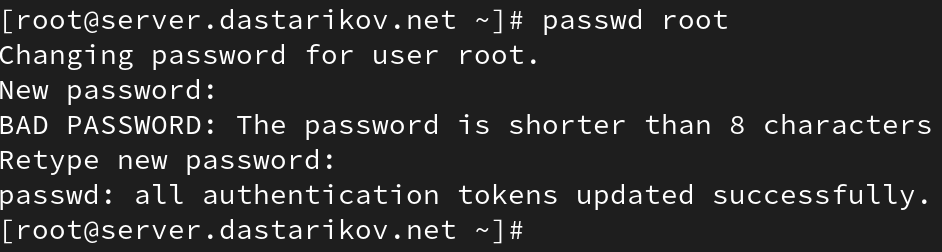
\includegraphics[width=\textwidth]{../images/image01.png}
  \captionof{figure}{Задание пароля для пользователя root.}
\end{frame}

\begin{frame}[fragile]
\frametitle{Запрет удалённого доступа по SSH для пользователя root}
Запретили пользователю root подключение к серверу через SSH:
  \begin{minted}{bash}
    PermitRootLogin no
  \end{minted}
  \centering
  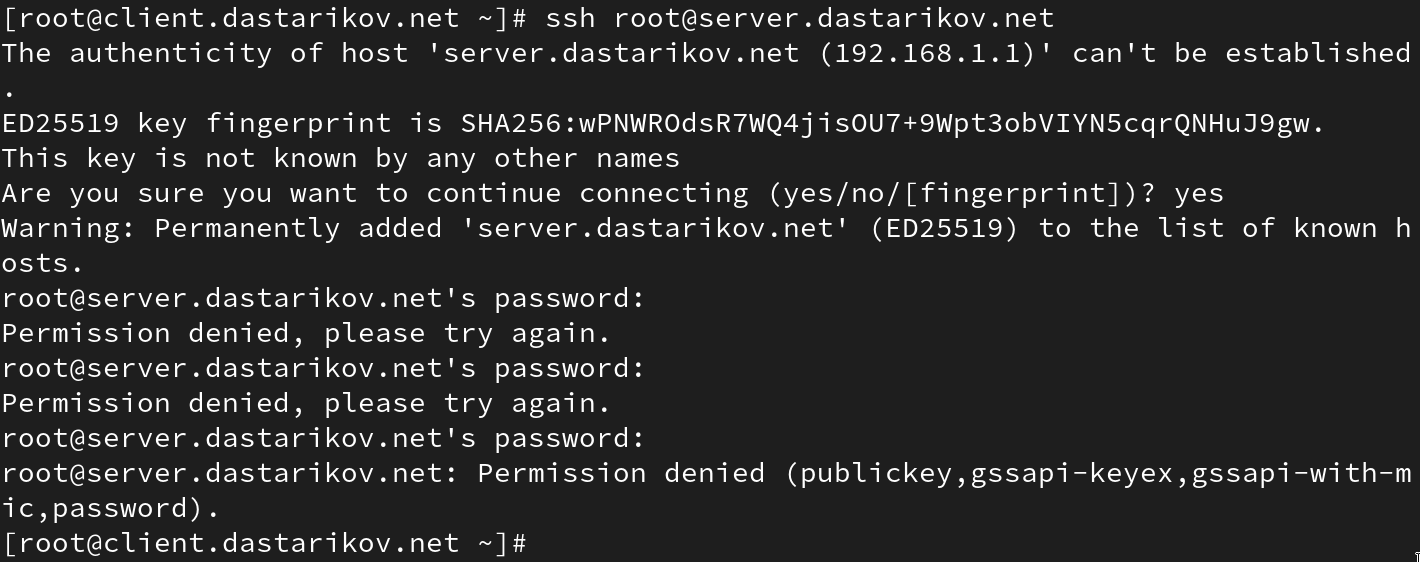
\includegraphics[width=\textwidth]{../images/image02.png}
  \captionof{figure}{Подключение к серверу через SSH-соединение.}
\end{frame}

\begin{frame}
\frametitle{Ограничение списка пользователей для удалённого доступа по SSH}
  \centering
  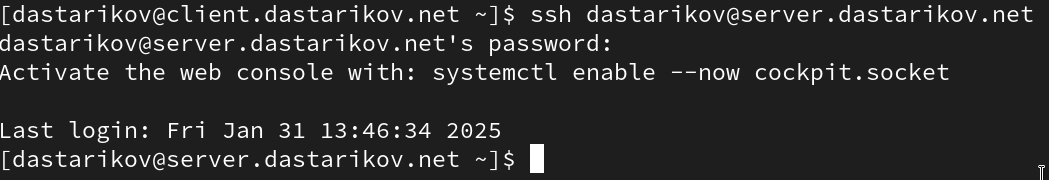
\includegraphics[width=\textwidth]{../images/image03.png}
  \captionof{figure}{Успешное подключение к серверу пользователем dastarikov.}
\end{frame}

\begin{frame}[fragile]
\frametitle{Ограничение списка пользователей для удалённого доступа по SSH}
Явно указали разрешенных к подключению пользователей:
  \begin{minted}{bash}
    AllowUsers vagrant
  \end{minted}
  \centering
  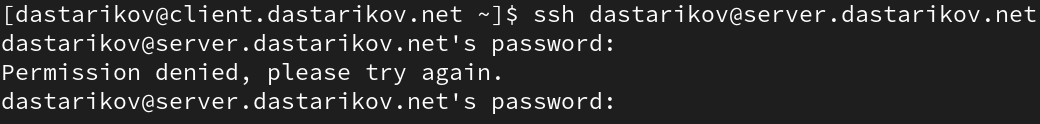
\includegraphics[width=\textwidth]{../images/image04.png}
  \captionof{figure}{Отказ в доступе на сервер пользователю dastarikov.}
\end{frame}

\begin{frame}[fragile]
\frametitle{Ограничение списка пользователей для удалённого доступа по SSH}
Обновили список разрешенных пользователей:
  \begin{minted}{bash}
    AllowUsers vagrant dastarikov
  \end{minted}
  \centering
  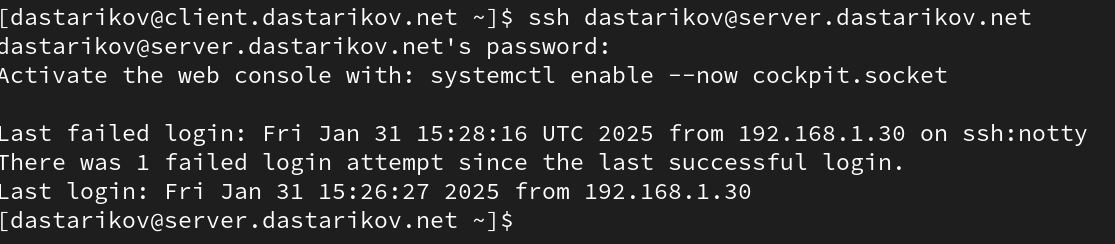
\includegraphics[width=\textwidth]{../images/image05.png}
  \captionof{figure}{Восстановление доступа на сервер пользователю dastarikov.}
\end{frame}

\begin{frame}[fragile]
\frametitle{Настройка дополнительных портов для удалённого доступа по SSH}
В файле конфигурации \texttt{sshd\_config} добавили строки:
  \begin{minted}{bash}
    Port 22
    Port 2022
  \end{minted}
  \centering
  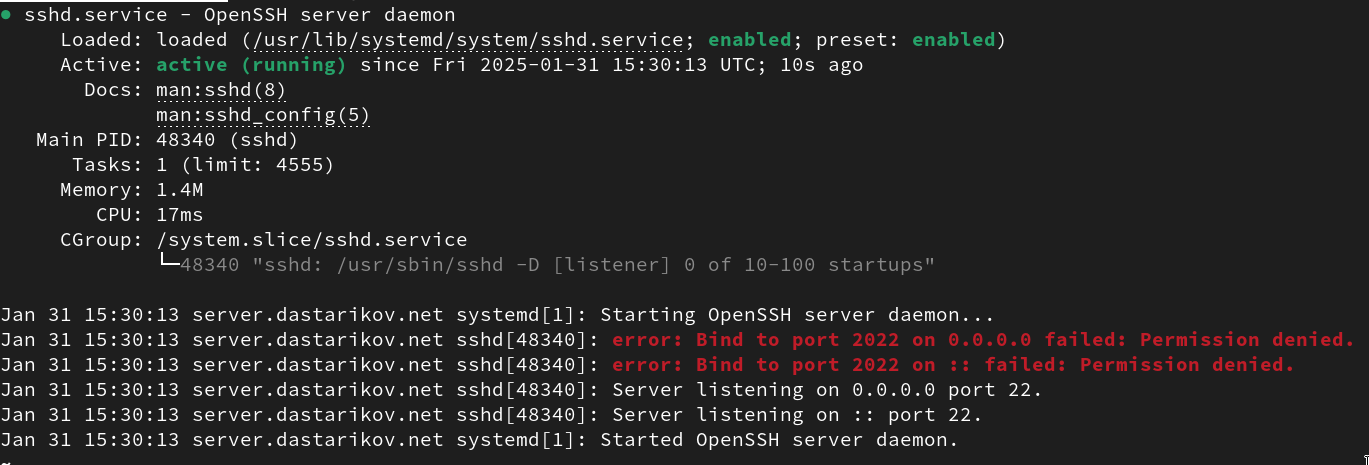
\includegraphics[width=\textwidth]{../images/image06.png}
  \captionof{figure}{Проверка расширенного статуса работы sshd.}
\end{frame}

\begin{frame}
\frametitle{Настройка дополнительных портов для удалённого доступа по SSH}
  \centering
  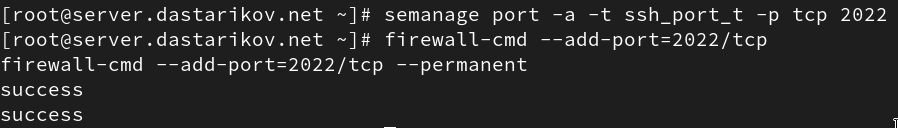
\includegraphics[width=\textwidth]{../images/image07.png}
  \captionof{figure}{Настройка межсетевого экрана.}
\end{frame}

\begin{frame}
\frametitle{Настройка дополнительных портов для удалённого доступа по SSH}
  \centering
  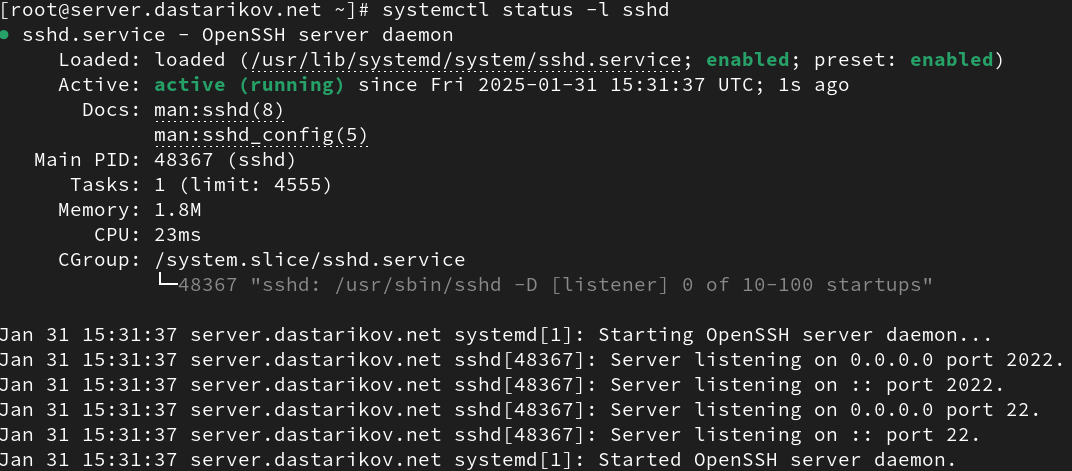
\includegraphics[width=\textwidth]{../images/image08.png}
  \captionof{figure}{Просмотр расширенного статуса sshd после настройки работы с портом 2022.}
\end{frame}

\begin{frame}
\frametitle{Настройка дополнительных портов для удалённого доступа по SSH}
  \centering
  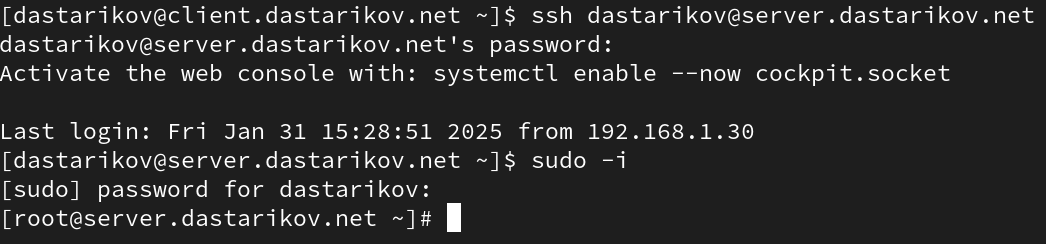
\includegraphics[width=\textwidth]{../images/image09.png}
  \captionof{figure}{Успешное подключение к серверу.}
\end{frame}

\begin{frame}
\frametitle{Настройка дополнительных портов для удалённого доступа по SSH}
  \centering
  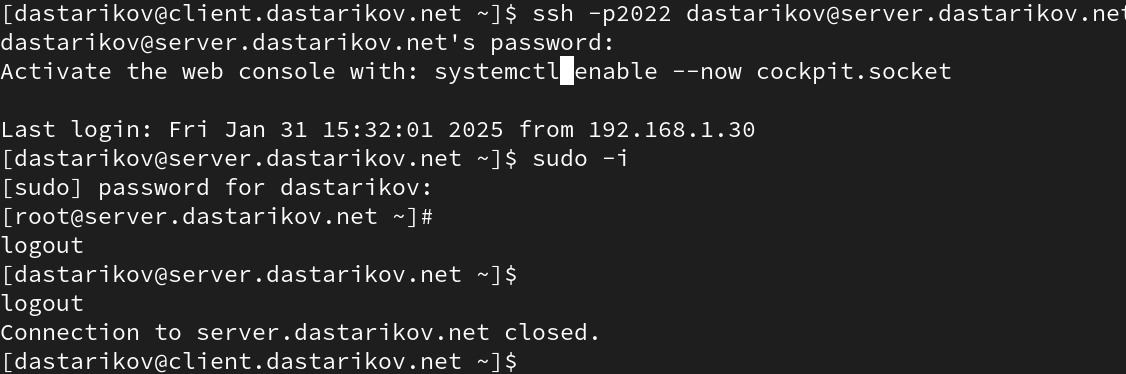
\includegraphics[width=\textwidth]{../images/image10.png}
  \captionof{figure}{Успешное подключение к серверу по порту 2022.}
\end{frame}

\begin{frame}
\frametitle{Настройка удалённого доступа по SSH по ключу}
  \centering
  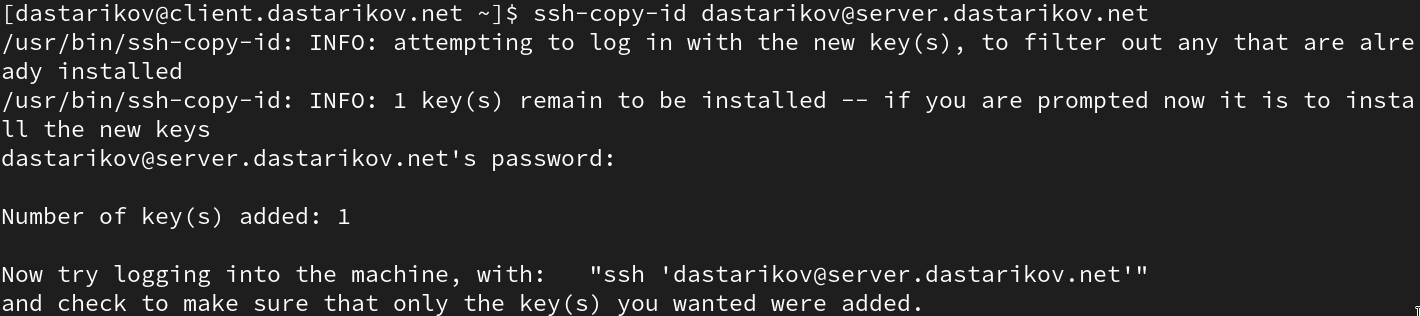
\includegraphics[width=\textwidth]{../images/image11.png}
  \captionof{figure}{Копирование открытого ключа на сервер.}
\end{frame}

\begin{frame}
\frametitle{Настройка удалённого доступа по SSH по ключу}
  \centering
  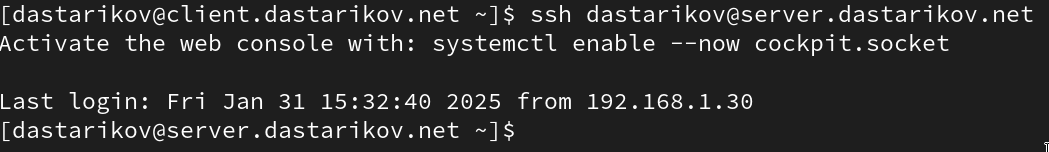
\includegraphics[width=\textwidth]{../images/image12.png}
  \captionof{figure}{Успешное подключение к серверу с использованием SSH-ключа.}
\end{frame}

\begin{frame}
\frametitle{Организация туннелей SSH, перенаправление TCP-портов}
  \centering
  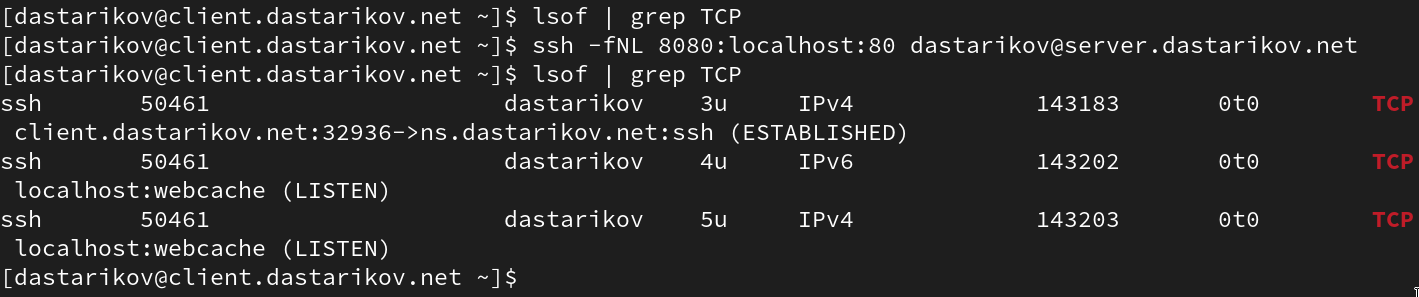
\includegraphics[width=\textwidth]{../images/image13.png}
  \captionof{figure}{Перенаправление TCP-портов.}
\end{frame}

\begin{frame}
\frametitle{Запуск консольных приложений через SSH}
  \centering
  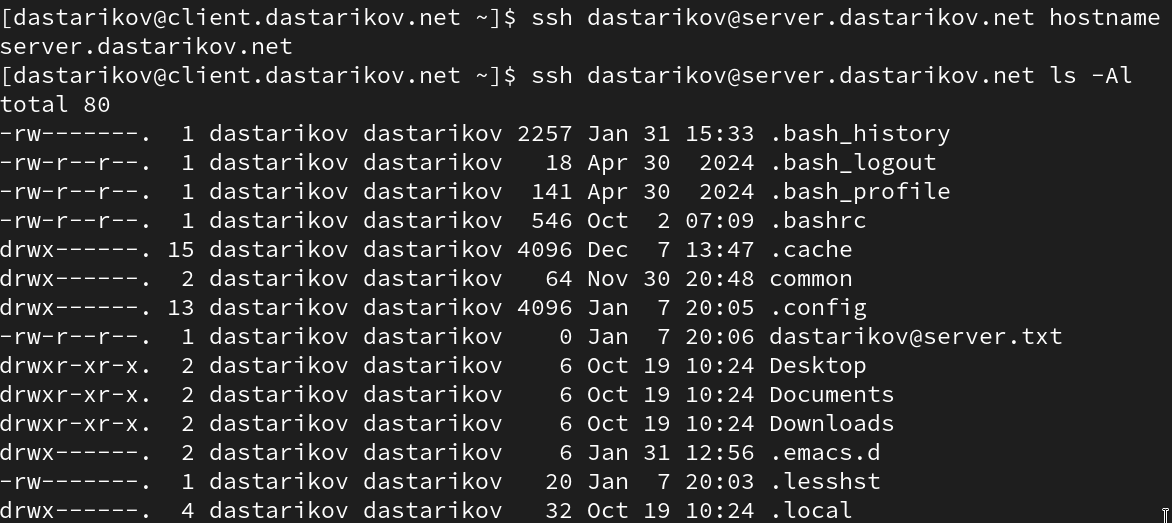
\includegraphics[width=\textwidth]{../images/image14.png}
  \captionof{figure}{Просмотр имени узла сервера и списка файлов через ssh.}
\end{frame}

\begin{frame}
\frametitle{Запуск консольных приложений через SSH}
  \centering
  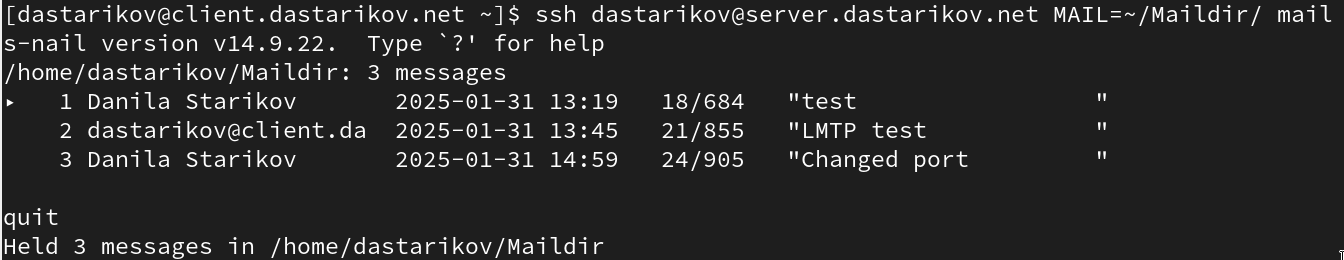
\includegraphics[width=\textwidth]{../images/image15.png}
  \captionof{figure}{Просмотр почты на сервере через ssh.}
\end{frame}

\begin{frame}[fragile]
\frametitle{Запуск графических приложений через SSH (X11Forwarding)}
Разрешили отображать на локальном клиентском компьютере графические интерфейсы X11:
  \begin{minted}{bash}
    X11Forwarding yes
  \end{minted}
Запустили графическое приложение на сервере:
  \begin{minted}{bash}
    ssh -YC dastarikov@server.dastarikov.net firefox
  \end{minted}
  \centering
  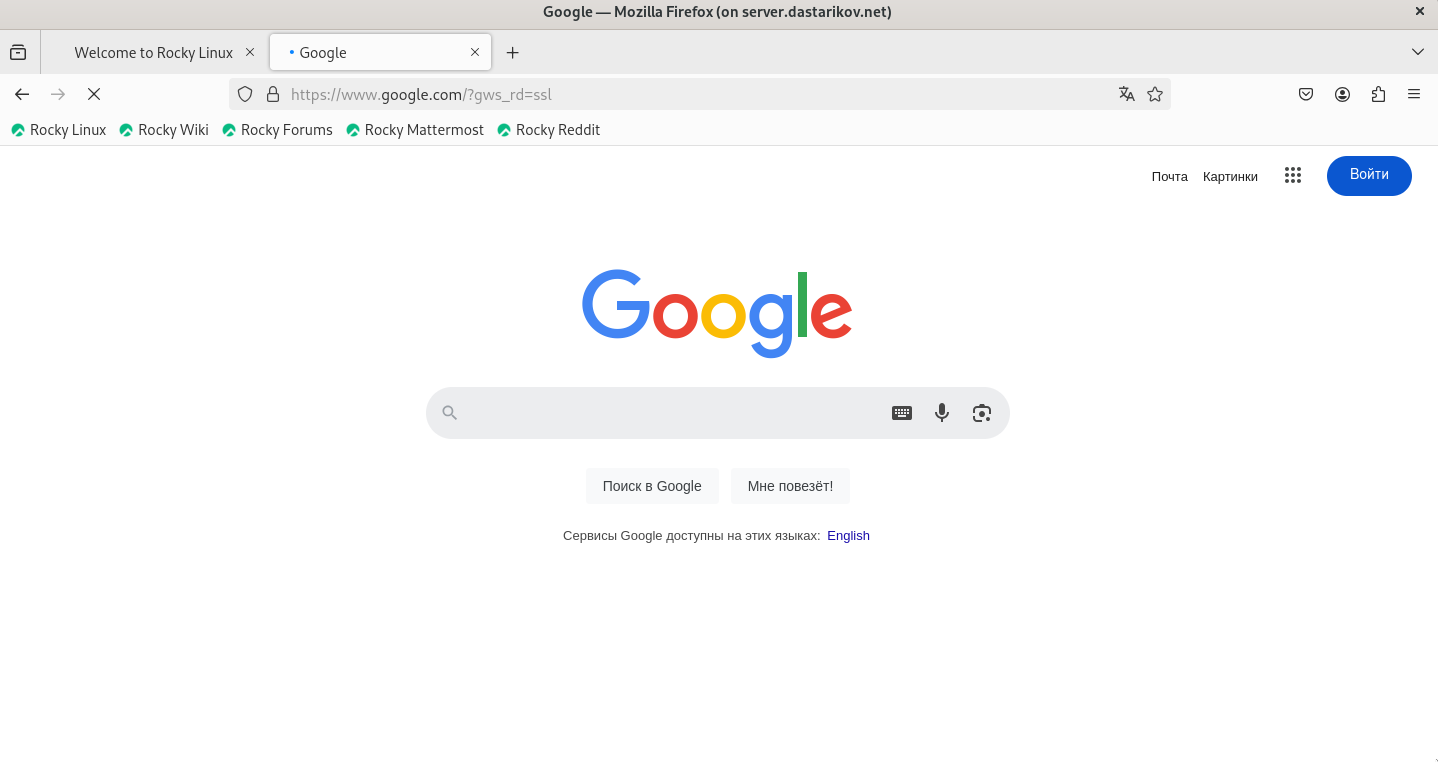
\includegraphics[width=0.7\textwidth]{../images/image16.png}
  \captionof{figure}{Просмотр графического приложения (firefox) через ssh.}
\end{frame}

\begin{frame}[fragile]
\frametitle{Внесение изменений в настройки внутреннего окружения виртуальной машины}
  \begin{minted}[breaklines]{bash}
    cd /vagrant/provision/server
    mkdir -p /vagrant/provision/server/ssh/etc/ssh
    cp -R /etc/ssh/sshd_config /vagrant/provision/server/ssh/etc/ssh/
    cd /vagrant/provision/server
    touch ssh.sh
    chmod +x ssh.sh
  \end{minted}
\end{frame}

\begin{frame}[fragile]
\frametitle{Внесение изменений в настройки внутреннего окружения виртуальной машины}
  \begin{minted}[breaklines]{bash}
    #!/bin/bash
    echo "Provisioning script $0"
    echo "Copy configuration files"
    cp -R /vagrant/provision/server/ssh/etc/* /etc
    restorecon -vR /etc
    echo "Configure firewall"
    firewall-cmd --add-port=2022/tcp
    firewall-cmd --add-port=2022/tcp --permanent
    echo "Tuning SELinux"
    semanage port -a -t ssh_port_t -p tcp 2022
    echo "Restart sshd service"
    systemctl restart sshd
  \end{minted}
\end{frame}


\begin{frame}[fragile]
\frametitle{Внесение изменений в настройки внутреннего окружения виртуальной машины}
\begin{minted}{bash}
    server.vm.provision "server ssh",
    type: "shell",
    preserve_order: true,
    path: "provision/server/ssh.sh"
\end{minted}
\end{frame}

\begin{frame}
\frametitle{Выводы}
\begin{itemize}
    \item В результате выполнения лабораторной работы приобрели практические навыки по настройке удалённого доступа к серверу с помощью SSH.
\end{itemize}
\end{frame}
\end{document}
